% This is "sig-alternate.tex" V2.0 May 2012
% This file should be compiled with V2.5 of "sig-alternate.cls" May 2012
%
% This example file demonstrates the use of the 'sig-alternate.cls'
% V2.5 LaTeX2e document class file. It is for those submitting
% articles to ACM Conference Proceedings WHO DO NOT WISH TO
% STRICTLY ADHERE TO THE SIGS (PUBS-BOARD-ENDORSED) STYLE.
% The 'sig-alternate.cls' file will produce a similar-looking,
% albeit, 'tighter' paper resulting in, invariably, fewer pages.
%
% ----------------------------------------------------------------------------------------------------------------
% This .tex file (and associated .cls V2.5) produces:
%       1) The Permission Statement
%       2) The Conference (location) Info information
%       3) The Copyright Line with ACM data
%       4) NO page numbers
%
% as against the acm_proc_article-sp.cls file which
% DOES NOT produce 1) thru' 3) above.
%
% Using 'sig-alternate.cls' you have control, however, from within
% the source .tex file, over both the CopyrightYear
% (defaulted to 200X) and the ACM Copyright Data
% (defaulted to X-XXXXX-XX-X/XX/XX).
% e.g.
% \CopyrightYear{2007} will cause 2007 to appear in the copyright line.
% \crdata{0-12345-67-8/90/12} will cause 0-12345-67-8/90/12 to appear in the copyright line.
%
% ---------------------------------------------------------------------------------------------------------------
% This .tex source is an example which *does* use
% the .bib file (from which the .bbl file % is produced).
% REMEMBER HOWEVER: After having produced the .bbl file,
% and prior to final submission, you *NEED* to 'insert'
% your .bbl file into your source .tex file so as to provide
% ONE 'self-contained' source file.
%
% ================= IF YOU HAVE QUESTIONS =======================
% Questions regarding the SIGS styles, SIGS policies and
% procedures, Conferences etc. should be sent to
% Adrienne Griscti (griscti@acm.org)
%
% Technical questions _only_ to
% Gerald Murray (murray@hq.acm.org)
% ===============================================================
%
% For tracking purposes - this is V2.0 - May 2012

\documentclass{sig-alternate}

\usepackage{fixme}
\fxsetup{
	status=draft,
	author=,
	layout=inline,
	theme=color
}
\usepackage{float}
\usepackage{amsmath}

\begin{document}
%
% --- Author Metadata here ---
\conferenceinfo{}{}
%\CopyrightYear{2007} % Allows default copyright year (20XX) to be over-ridden - IF NEED BE.
%\crdata{0-12345-67-8/90/01}  % Allows default copyright data (0-89791-88-6/97/05) to be over-ridden - IF NEED BE.
% --- End of Author Metadata ---

\title{Drummer: Probing and Hearing your Location}

%
% You need the command \numberofauthors to handle the 'placement
% and alignment' of the authors beneath the title.
%
% For aesthetic reasons, we recommend 'three authors at a time'
% i.e. three 'name/affiliation blocks' be placed beneath the title.
%
% NOTE: You are NOT restricted in how many 'rows' of
% "name/affiliations" may appear. We just ask that you restrict
% the number of 'columns' to three.
%
% Because of the available 'opening page real-estate'
% we ask you to refrain from putting more than six authors
% (two rows with three columns) beneath the article title.
% More than six makes the first-page appear very cluttered indeed.
%
% Use the \alignauthor commands to handle the names
% and affiliations for an 'aesthetic maximum' of six authors.
% Add names, affiliations, addresses for
% the seventh etc. author(s) as the argument for the
% \additionalauthors command.
% These 'additional authors' will be output/set for you
% without further effort on your part as the last section in
% the body of your article BEFORE References or any Appendices.

% \numberofauthors{8} %  in this sample file, there are a *total*
% of EIGHT authors. SIX appear on the 'first-page' (for formatting
% reasons) and the remaining two appear in the \additionalauthors section.
%
\author{
% You can go ahead and credit any number of authors here,
% e.g. one 'row of three' or two rows (consisting of one row of three
% and a second row of one, two or three).
%
% The command \alignauthor (no curly braces needed) should
% precede each author name, affiliation/snail-mail address and
% e-mail address. Additionally, tag each line of
% affiliation/address with \affaddr, and tag the
% e-mail address with \email.
%
% 1st. author
\alignauthor
Kaifei Chen, Beidi Chen, Randy Katz, David Culler\\
\affaddr{Computer Science Division}\\
\affaddr{University of California, Berkeley}\\
\email{\{kaifei, beidic, randy, culler\}@cs.berkeley.edu}
}
% There's nothing stopping you putting the seventh, eighth, etc.
% author on the opening page (as the 'third row') but we ask,
% for aesthetic reasons that you place these 'additional authors'
% in the \additional authors block, viz.
% \additionalauthors{Additional authors: John Smith (The Th{\o}rv{\"a}ld Group,
% email: {\texttt{jsmith@affiliation.org}}) and Julius P.~Kumquat
% (The Kumquat Consortium, email: {\texttt{jpkumquat@consortium.net}}).}
% \date{30 July 1999}
% Just remember to make sure that the TOTAL number of authors
% is the number that will appear on the first page PLUS the
% number that will appear in the \additionalauthors section.
\maketitle
\begin{abstract}
Abstract
\end{abstract}

% A category with the (minimum) three required fields
% \category{H.4}{Information Systems Applications}{Miscellaneous}
% %A category including the fourth, optional field follows...
% \category{D.2.8}{Software Engineering}{Metrics}[complexity measures, performance measures]

% \terms{System, Deployment, Data analysis}

% \keywords{Semantic localization, Machine learning}

\section{Introduction}
\label{sec:intro}


Indoor localization enables plenty of location-based applications. 




People has been attempting indoor localization in a wide scope of approaches, ranging from 
trilateration to fingerprinting to dead reckoning. Inertial measurement units (IMU), 
mostly referring accelerometer, 
compass, and gyroscope, have been ubiquitous with the explosion of mobile phones, and used in
estimating in-building trajectories for localization. However, because of hardware limitation, 
IMU in mobile phone suffer from drift and cumulative errors. 



% we need semantic location
However, the focuses of these work are not perfectly in line with requirements from location-based services (LBS). 
Most of them are purely focusing on how to localize a geometric location, whereas 
many indoor LBS also requires the semantic of the location rather than the location itself, such as room number,
or a handicap door. \fxnote{say geometric is important, interaction, proximity social network} 
One example of indoor LBS is occupancy driven HVAC (heating, ventilation, and air conditioning).
Because HVAC control are at most room-level granularity, so estimating the number of room the 
user is in will be more nature and helpful. For LBSs that requires geometric locations, semantic will also help
in many cases. For instance, proximity based social network \fxnote{[cite]} need to ensure two people staying near
to each other have no wall in between. 



% \fxnote{geometric location needs calibration}
Geometric location can be done by: trilateration or triangulation, dense site survey + fingerprinting, dead reckoning.
First one doesn't work because of obstacles, second doesn't work because training overhead. 3rd works, but it needs calibration. 
step count, particle filter, kalman filter.


Location semantics can be inferred in different approaches. One way is to get geometric location with 
adequate accuracy. By using predefined location to semantic information database \fxnote{[cite]}, we can get semantic information
by querying geometric locations, which is also adopted by the majority of outdoor location-based services.
However, given much richer information and faster environment change, creating and maintaining such as a
semantic database is not feasible in most buildings. On the other hand, many semantic information requires
find grained geometric estimation that can hardly be archived by state-of-art localization techniques. For 
example, energy foot-printing \fxnote{[cite]} is the notion of monitoring personal energy consumption
according to her location and 
the electronic devices (e.g. coffee machine, refrigerator, microwave) being used at that location. The 
distance between these devices can be sub-meter, and no current geometric localization technique can achieve this 
accuracy in general cases. Another idea to infer semantic location is from the physical features, and it is very application
specific. For instance, a room is usually enclosed by walls, so you should be able to encode room number in 
special light bulbs, and give perfect room-level localization. However, some office buildings use glasses to separate
rooms. %Also ultrasound beacon may also work, but some buildings has no door 
For energy foot-printing, one can actually either see (by camera) or hear (by microphone) what the user is doing.



% intro of Drummer
In this paper, we introduce {\em Drummer}, a environment probing and listening service 
to assist both geometric calibration and semantic indoor localization inference. The basic idea is sound 
can be used to measure distance from walls, and also learn human activities that will create featured sound.
This solve all problems, because: it can 
provide continuous calibration, it can detect environment change, 
it provide room level fingerprining, sound has plenty potential of inferring activity (fridge/coffee machine).


In summary, our contributions are: (i) it can provide continuous calibration. (ii) it can detect environment change. 
(iii) it provide room level fingerprining. (iv) sound has plenty potential of inferring activity (fridge/coffee machine).
(v) provide huge potential for extension and improvements

Roadmap: Section 2 related work and their faults, Section 3 overview, Section 4 calibrations, Section 5 Physical inference, 
Section 6 evaluation. Section 7 Discussion. Section 8 Conclusion

% % acoustic signal was used a lot for environment detection
% Audio probing has been used for tens of years in various ways to help indirectly
% inspect environments or objects. Sonar is used by vessels to leverage sound propagation 
% time to detect underwater objects. Ultrasonography uses ultrasound to generate
% diagnostic imaging of subcutaneous body structures in clinics. \fxnote{more use cases}
% Given the physical attributes of audio signal, it is idea for use in environment detection.
% Sound wave is longitudinal mechanical wave, so \fxnote{what?}. 


% % acoustic signal should be used for environment detection but not
% With ubiquitous audio devices (e.g.\ microphone and speaker) built in all phones, 
% acoustic signal should also be used for 
% environment detection as an service. Applications including indoor localization, occupancy detection,
% and 3D model reconstruction, can benefit from the feedback of this service.
% However, acoustic devices in mobile phones gain little attention in 
% industry and have not been evolved as much as other components \cite{invensense, applem7} 
% in terms of providing physical information.
% Most acoustic applications is focusing on semantic information in voice, such as natural 
% language processing and text-to-speech synthesis. These areas require only audible
% sounds with adequate 
% accuracy, and have good baseline proof of feasibility that human brain can process it
% \cite{nirjon2013auditeur}.
% Whereas smart phones haven't made the step to evolve from a phone to a smart 
% mobile device that could converts physical information into cyber world using acoustic signal. 
% Worse still, most phones do audible sound specific optimizations in operating systems or 
% hardware firmware, and provide no access to the raw audio data. Specifically, mobile phone
% tend to audio noise cancellation for communication and entertainment quality, which makes 
% it impossible to record the sound sent by itself in application layer.


% % current work on audio probing 
% In spite of these impediments, several recent work has been done on inferring physical world 
% information using acoustic signal feature. Examples include: gesture detection using Doppler effect
% \cite{gupta2012soundwave, sun2013spartacus}, room shape reconstruction using echo \cite{dokmanic2013acoustic}, 
% blah
%  \fxnote{details about those work}


% % our work
% In this paper, we introduce {\em Drummer} - a mobile could service to enable several environment awareness 
% features using acoustic signal. \fxnote{goal, arch, algorithm}



% % summary
% In summary, our contributions are:

% \begin{itemize}

% \item Propose several environment detection features and their algorithms.

% \item Investigate how good we can get for each feature, and advocate industry to enable 
% more raw information from hardware layer, and expand the functionality of audio devices, 
% such as maximum sending and sampling frequency.

% \end{itemize}


% % roadmap


% To learn the environment, computer vision techniques has been proposed to capture 
% and reconstruct things from video and images, such as objects 
% \cite{rothganger20063d}, scenes \cite{snavely2006photo}, and buildings 
% \cite{furukawa2009reconstructing}. These techniques require fairly amount of 
% data and heavy post-processing computation. In addition, depth information from 
% RGB-D cameras are used to enable interactive real time 3D visual modeling, 
% especially while RGB-D sensors are getting cheaper, such as Microsoft Kinect 
% \cite{du2011interactive, izadi2011kinectfusion}.


% However, RGB-D cameras are still not available for most people. And privacy 
% concerns could be raised when reconstructing visual model of open spaces, 
% especially in indoor environment, where private information can be more 
% heterogeneous compared to outdoor situation. More importantly, not all 
% applications actually require accurate and complete model of environment. 
% For example, with the knowledge of floor plan, we can infer what a person 
% is doing simply by acquiring a coarse estimation of her/his location. 
%Standing in front of projection screen implies she/he is presenting, 


% We propose to use acoustic echo to probe the environment, and build coarse 3D model 
% of the environment. Microphones and speakers are available on almost all phones, 
% which makes crowd-sourcing possible. And 
% sensing the echo of a sound pulse will bring up almost no privacy concerns. We are 
% trying to look at how accurate we can achieve to reconstruct 3D in-room model, and 
% how much benefits we can introduce to existing techniques.


% 3D modeling/inroom localization

% We only focus on closed environment

% Video: Privacy, Energy Consumption, Computation, Availability

\section{Related Work}
\label{sec:related}



\subsubsection{Zee}
It use trajectory on map to do enhanced particle filter


Room is not accesable on map, no specific trajectory in room


we can locate in room
we can hear



\subsubsection{Walkie Markie}
Only works when router is on hallway.



\subsubsection{UnLoc}
Too oppotunistic
No Fingerprint guarantee



\subsubsection{SLAM}

no camera, no laser


% BeepBeep, accurate phone-to-phone ranging\cite{peng2007beepbeep}


% Relative Phone localization \cite{qiu2011feasibility} 


% PNAS \cite{dokmanic2013acoustic} use several microphone to determine the shape of a room.


% ultrasound imaging \cite{}.



% Losts of localization, using ultrasound \cite{harter2002anatomy}, \cite{priyantha2000cricket}.
%\section{Challenges}
\label{sec:chall}

To leverage information from sound using commercial smartphones, we need to
tackle several challenges from different aspects. In this section we 


\subsection{Hardware Limitation on Mobile Phones}

frequency limit
accuracy limit


\subsection{Systematic Error from Hardware}
Commercial hardware may have large systematic errors. 
Given the use cases, off-the-shelf smartphones usually don't use expensive
speaker and microphone. Therefore we expect relatively high systematic error 
using these acoustic sensors. Accurate signal processing techniques, such as 
cross-correlation, will be less effective and may introduce more bias or noise.


\fxnote{Add a graph showing collected sound and theoretical sound, and 
show their diff, along time axis}

To show how much this problem will influence our result, we send exponential chirp 
in a outdoor open space Figure x, 


\subsection{Environmental Noise}


\subsection{Information Inference}
Hard to model physical responses


%To achieve the final goal of reconstructing 3D environment model, 
%we need to measure distances of different objects (e.g. walls, desks, chairs).
%The first problem to tackle is to measure distance from a single wall. 
%For example, how to measure or determine the echo in the recorded audio trace?
% 
% 
% \subsubsection{Multiple Distance Measurement}
% 
% Then we need to generalize the distance measurements to closed environment 
% where reflections and multi-path can bring lost of noise.
% 
% 
% \subsubsection{Direction Identification}
% 
% Besides the distance of objects around the phone, knowing the direction of the 
% object is also very crucial to build the 3D model. 

\section{Drummer Overview}
\label{sec:overview}


\begin{figure}[H]
\centering
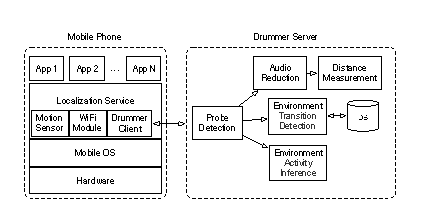
\includegraphics[width=0.45\textwidth]{./fig/arch.eps}
\caption{System Architecture of Drummer \fxnote{am I mixing arch and algorithm here?}}
\label{fig:arch}
\end{figure}


The system archtecture of Drummer is shown in figure \ref{fig:arch}. The mobile phone drummer 
client keeps minimum work and offloads data and computation to the cloud. In this paper, we assume 
network connectivity are awalys sufficient to stream audio data. Tackling with bad network conditions 
\cite{cuervo2010maui} and optimizing audio streaming \cite{farleycsense} are also important 
problems, but they are outside the scope of this paper. A drummer server maintains a TCP connection
with each client for upstream audio streaming and downstream event-based environmental information
retrieved from sound. The drumer server implements all algorithms we will discuss in next section.


\subsection{Mobile Phone Client}

The mobile phone drumer client sits in between mobile phone operating system and applications.
It provides asynchronize APIs for applications to get updates of the latest estiamted features of
current spatial environment. The current proposed and implemented features are discusses in next section.
The client initializes a TCP connection to server, keeps streaming the audio data to Drummer server, 
and receives different types of environmental features, as described next.



\subsection{Drummer Server}

Server is 
\section{Geometric Location}
\label{sec:geo}

Geometric localization aims to pinpoint the target. This can be done either by 
inferring relative spacial relationship to beacons or fingerprints, or dead-reckoning


\subsection{Distance from Nearest Walls}

Geometric information can be obtained from measuring Round Trip Time (RTT)
of a probing chirp. 

\subsubsection{Chirp}


sweep frequency chirp


Select Chirp Amplitude and Frequency

We firstly measure the ambient sound, and choose a quiet frequency.


What is chirp


why chirp?


How to generate chirp?


What chirp to use?


How to see echo? Time delay of echo, Shape of echo pulse, Phase Diff


SNR etc.

\fxnote{GRAPH: chirp and echo shape}

\subsubsection{Recording}

\subsubsection{Cross-correlation and Audio Reduction}

After receiving the original sound and echo, we do auto-correlation with original sound,
and remove it from the audio track.

\fxnote{GRAPH: how auto-correlation works}


\subsubsection{Locating Echoes}

Envelop is the sound of big surface. Physical explanation. 
Define envelop as the same duration of original sound.



\begin{figure}[H]
\centering
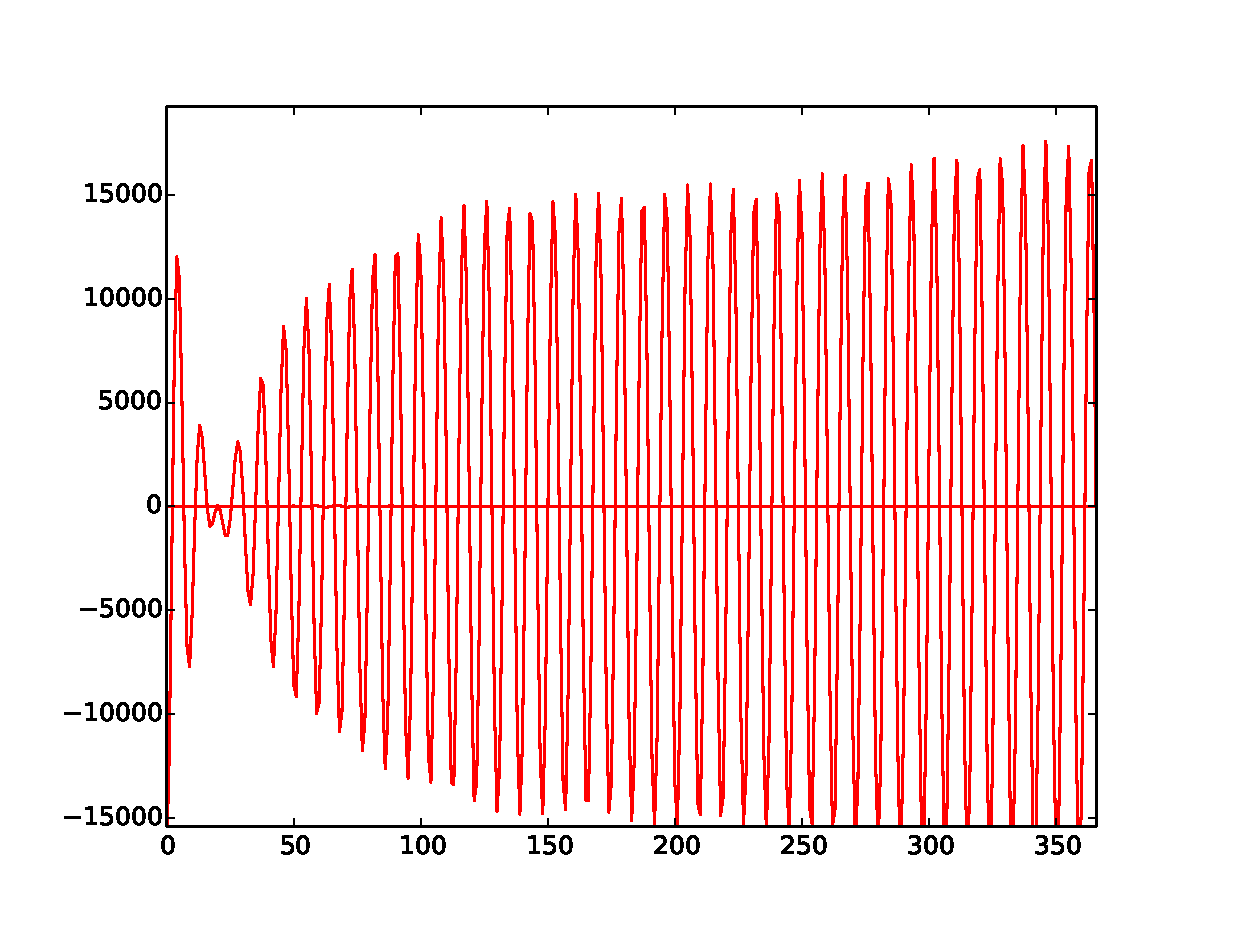
\includegraphics[width=0.45\textwidth]{./fig/20cm.eps}
\caption{20cm from wall, 50ms chirp}
\end{figure}

\begin{figure}[H]
\centering
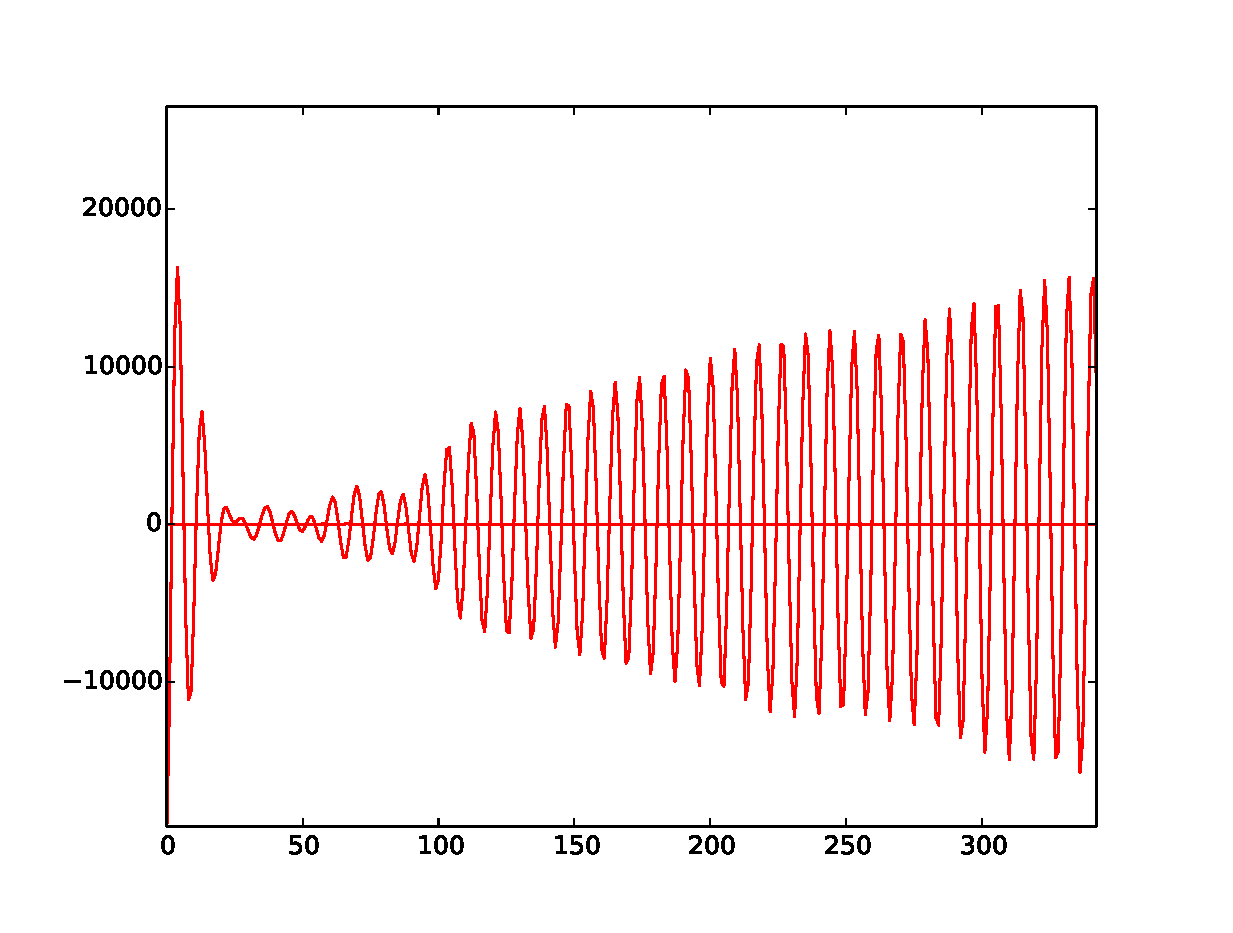
\includegraphics[width=0.45\textwidth]{./fig/40cm.eps}
\caption{40cm from wall, 50ms chirp}
\end{figure}

\begin{figure}[H]
\centering
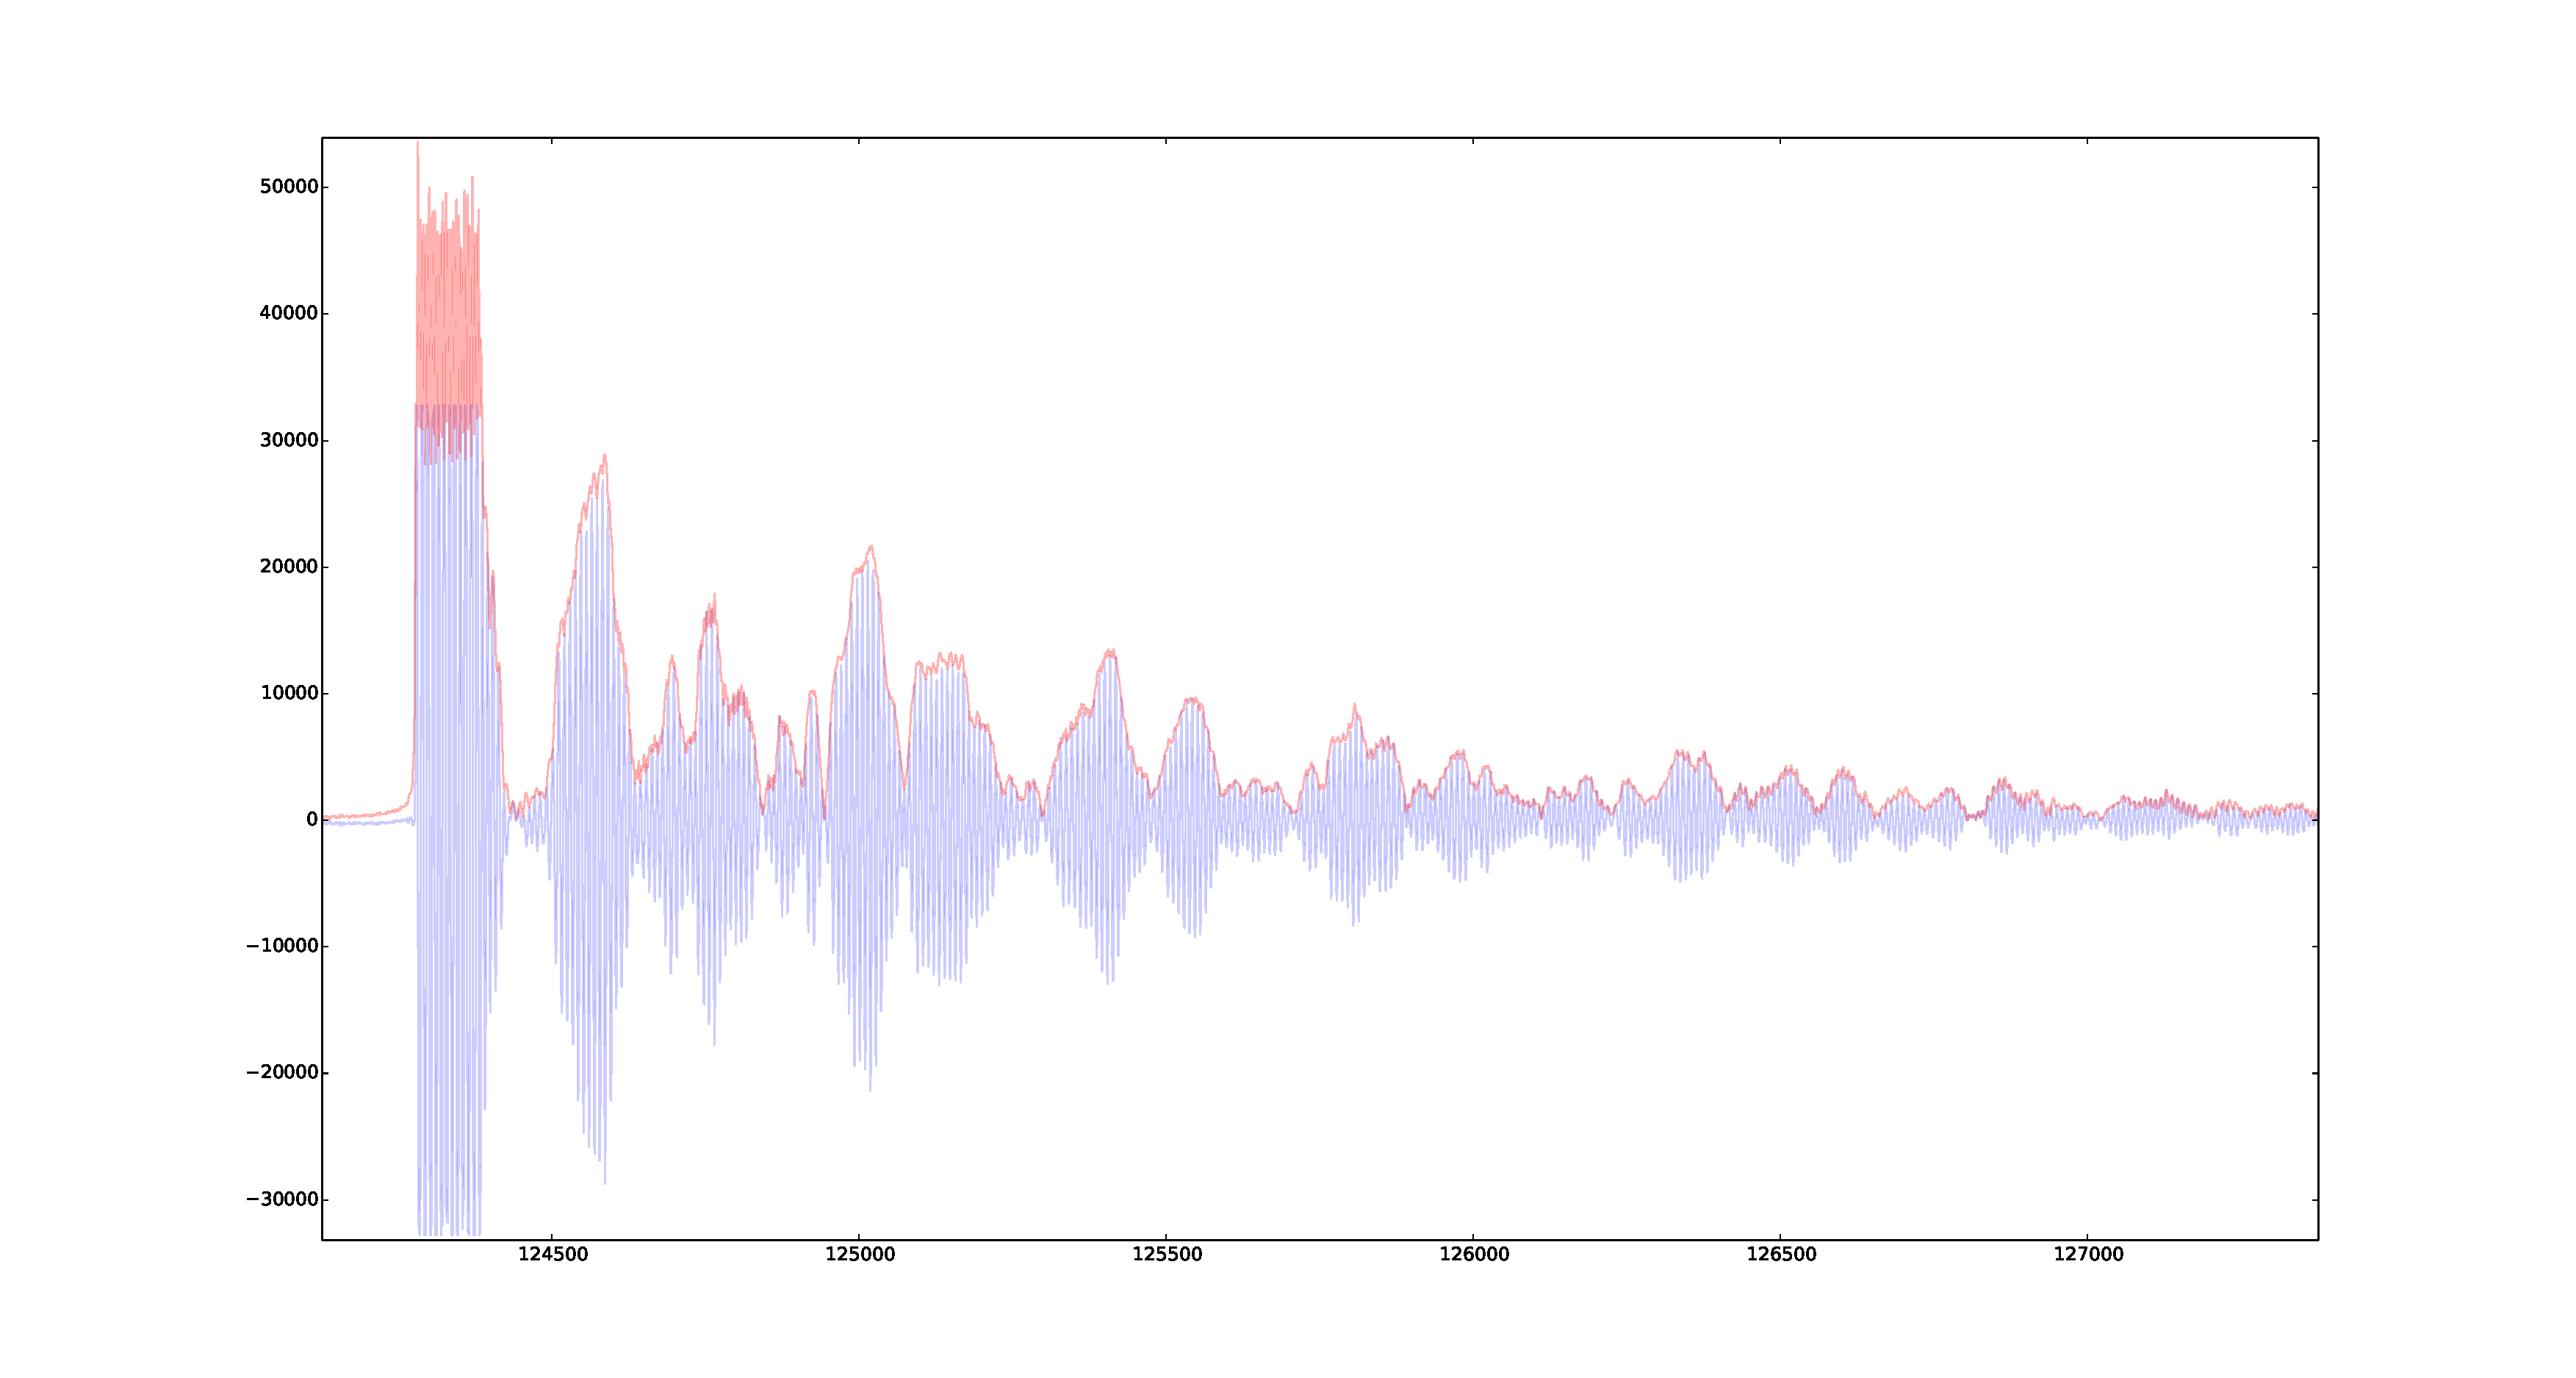
\includegraphics[width=0.45\textwidth]{./fig/inroom.pdf}
\caption{40cm from wall, 5ms chirp}
\end{figure}



% \subsubsection{Phase Diff}



% \subsubsection{Shape of Echo}


% \subsubsection{Iterative Audio Reduction}

% We remove the acoustic effects of an object after determining its existence, and 
% in turn investigate the remaining sound iteratively. 


\subsection{Orientations of All Echoes}

We use TDoA of envelops to different microphones to determine the direction 
of the object represented by the envelop.


Binaural beat


\section{Semantic Location}
\label{sec:sem}

Aside from geometric locations, location semantics are usually more desired by applications.
Imaging a occupancy-driven HVAC controlling system, it is more preferable to locate a person 
at the other corner of the same room she is in, than a nearer point in the adjacent room. Also,
Knowing a person is using a coffee machine or microwave is more interesting than in front of which 
one she is standing. Generally speaking, activity are heavily inter-weaved with localization.
In this section, we propose to use sound to extend the ability to determine transitions of rooms 
of user, as well as sound-based activity recognitions.


\subsection{Environment Transition Detection}
\begin{figure}[H]
\centering
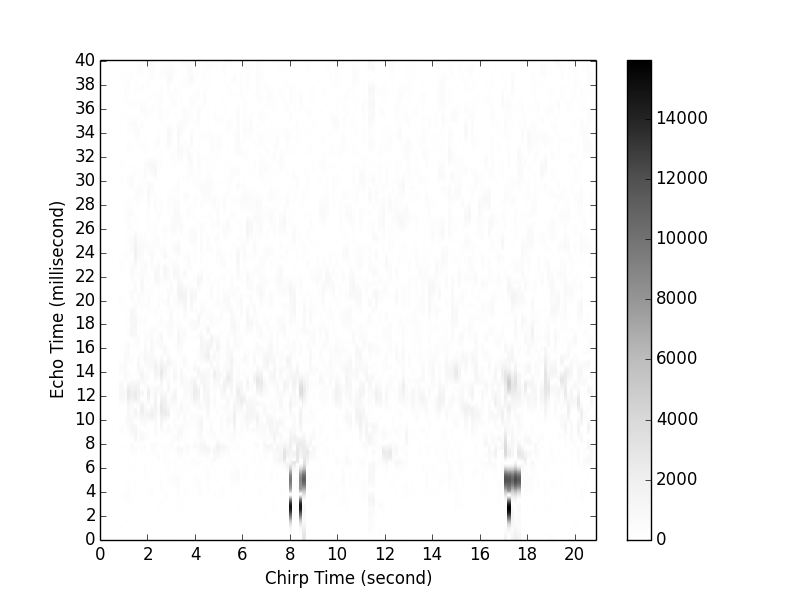
\includegraphics[width=0.45\textwidth]{./fig/transition.png}
\caption{Door Event}
\end{figure}


Rooms mostly come with physical walls in between, particularly when there is demand for 
room-level applications or services, such as room temperature or lighting control. Inferring and 
detecting room transition should be an essential functionality in indoor localization service.
Sound echo is ideal to detect the user going though a wall, which will cause a sudden environment 
change and also acoustic echo pattern change.


Drummer enables continuous environment probing when accelerometer data shows the person is moving.
 


The pattern of 
echoes will have a sudden change when walking through a door or corner.



\subsubsection{Spatial Environment Pattern}

ABS, coffee machine, fridge 
\section{Evaluation}
\label{sec:eval}

\subsection{Implementation Details}

Off-The-Shelf speaker cannot send large range chirp


Android Phone cannot send and listen. We use two phones to emulate.



\subsection{Distance Measurement}

\fxnote{GRAPH: accuracy, consistency at different distance, orientation}


% \subsection{In-room Ranging}

% \fxnote{GRAPH: accuracy at different locations in different size of rooms}


% \subsection{3D Modeling}


% \fxnote{GRAPH: 3D room map and 3D model}


\subsection{Room Change Detection}

\fxnote{GRAPH: true positive, false positive number}


\subsection{Localization}

Application includes location-based activity recognition

Activity inference based on location. Such as watching TV on couch, working on desk, sleeping on bed.


\subsection{Human Environment Interaction}
\section{Future Work}
\label{sec:future}


Phone Array over time, or use two MIC on a Phone to determine source of sound.
\section{Conclusions}
\label{sec:conclusions}

In this paper, 
%\end{document}  % This is where a 'short' article might terminate

%ACKNOWLEDGMENTS are optional
%\section{Acknowledgments}

%
% The following two commands are all you need in the
% initial runs of your .tex file to
% produce the bibliography for the citations in your paper.
\bibliographystyle{abbrv}
\bibliography{drummer}  % drummer.bib is the name of the Bibliography in this case
% You must have a proper ".bib" file
%  and remember to run:
% latex bibtex latex latex
% to resolve all references
%
% ACM needs 'a single self-contained file'!
%

% That's all folks!
\end{document}
